% Options for packages loaded elsewhere
\PassOptionsToPackage{unicode}{hyperref}
\PassOptionsToPackage{hyphens}{url}
%
\documentclass[
]{article}
\usepackage{amsmath,amssymb}
\usepackage{lmodern}
\usepackage{iftex}
\ifPDFTeX
  \usepackage[T1]{fontenc}
  \usepackage[utf8]{inputenc}
  \usepackage{textcomp} % provide euro and other symbols
\else % if luatex or xetex
  \usepackage{unicode-math}
  \defaultfontfeatures{Scale=MatchLowercase}
  \defaultfontfeatures[\rmfamily]{Ligatures=TeX,Scale=1}
\fi
% Use upquote if available, for straight quotes in verbatim environments
\IfFileExists{upquote.sty}{\usepackage{upquote}}{}
\IfFileExists{microtype.sty}{% use microtype if available
  \usepackage[]{microtype}
  \UseMicrotypeSet[protrusion]{basicmath} % disable protrusion for tt fonts
}{}
\makeatletter
\@ifundefined{KOMAClassName}{% if non-KOMA class
  \IfFileExists{parskip.sty}{%
    \usepackage{parskip}
  }{% else
    \setlength{\parindent}{0pt}
    \setlength{\parskip}{6pt plus 2pt minus 1pt}}
}{% if KOMA class
  \KOMAoptions{parskip=half}}
\makeatother
\usepackage{xcolor}
\usepackage[margin=1in]{geometry}
\usepackage{longtable,booktabs,array}
\usepackage{calc} % for calculating minipage widths
% Correct order of tables after \paragraph or \subparagraph
\usepackage{etoolbox}
\makeatletter
\patchcmd\longtable{\par}{\if@noskipsec\mbox{}\fi\par}{}{}
\makeatother
% Allow footnotes in longtable head/foot
\IfFileExists{footnotehyper.sty}{\usepackage{footnotehyper}}{\usepackage{footnote}}
\makesavenoteenv{longtable}
\usepackage{graphicx}
\makeatletter
\def\maxwidth{\ifdim\Gin@nat@width>\linewidth\linewidth\else\Gin@nat@width\fi}
\def\maxheight{\ifdim\Gin@nat@height>\textheight\textheight\else\Gin@nat@height\fi}
\makeatother
% Scale images if necessary, so that they will not overflow the page
% margins by default, and it is still possible to overwrite the defaults
% using explicit options in \includegraphics[width, height, ...]{}
\setkeys{Gin}{width=\maxwidth,height=\maxheight,keepaspectratio}
% Set default figure placement to htbp
\makeatletter
\def\fps@figure{htbp}
\makeatother
\setlength{\emergencystretch}{3em} % prevent overfull lines
\providecommand{\tightlist}{%
  \setlength{\itemsep}{0pt}\setlength{\parskip}{0pt}}
\setcounter{secnumdepth}{5}
\usepackage{lineno}
\linenumbers
\usepackage{float}
\usepackage{booktabs}
\usepackage{longtable}
\usepackage{array}
\usepackage{multirow}
\usepackage{wrapfig}
\usepackage{colortbl}
\usepackage{pdflscape}
\usepackage{tabu}
\usepackage{threeparttable}
\usepackage{threeparttablex}
\usepackage[normalem]{ulem}
\usepackage{makecell}
\usepackage{xcolor}
\ifLuaTeX
  \usepackage{selnolig}  % disable illegal ligatures
\fi
\usepackage[]{natbib}
\bibliographystyle{plainnat}
\IfFileExists{bookmark.sty}{\usepackage{bookmark}}{\usepackage{hyperref}}
\IfFileExists{xurl.sty}{\usepackage{xurl}}{} % add URL line breaks if available
\urlstyle{same} % disable monospaced font for URLs
\hypersetup{
  pdftitle={Aquifer depletion exacerbates agricultural drought losses in the US High Plains},
  pdfauthor={Taro Mieno; Timothy Foster; Shunkei Kakimoto; Nicholas Brozovic},
  hidelinks,
  pdfcreator={LaTeX via pandoc}}

\title{Aquifer depletion exacerbates agricultural drought losses in the US High Plains}
\author{}
% \author{Taro Mieno\footnote{Department of Agricultural Economics, University of Nebraska Lincoln, \href{mailto:tmieno2@unl.edu}{\nolinkurl{tmieno2@unl.edu}}} \and Timothy Foster\footnote{Department of WWW, University of Manchester, \href{mailto:timothy.foster@manchester.ac.uk}{\nolinkurl{timothy.foster@manchester.ac.uk}}} \and Shunkei Kakimoto\footnote{Department of Applied Economics, University of Minnesota, \href{mailto:kakim002@umn.edu}{\nolinkurl{kakim002@umn.edu}}} \and Nicholas Brozovic\footnote{Department of Agricultural Economics, University of Nebraska Lincoln, \href{mailto:nbrozovic@nebraska.edu}{\nolinkurl{nbrozovic@nebraska.edu}}}}
\date{}

\begin{document}
\maketitle
\begin{abstract}
Aquifer depletion poses a major threat to the ability of farmers, food supply chains, and rural economies globally to use groundwater as a means of adapting to climate variability and change. Empirical research has demonstrated the large differences in drought risk exposure that exist between rainfed and irrigated croplands, but previous work commonly assumes water supply for the latter is unconstrained. In this paper, we evaluate how aquifer depletion affects the resilience of irrigated crop production to drought risk using over 30 years of data on historical corn and soybean yields, production areas, and aquifer conditions for the High Plains region in the United States. We show that aquifer depletion reduces the ability of farmers to sustain irrigated crop yields and production areas in years and locations with large growing season water deficits. Our findings demonstrate that drought-related production losses on irrigated croplands increase non-linearly with aquifer depletion, highlighting the need for proactive aquifer conservation interventions to support adaptation and resilience to future increases in rainfall variability under climate change.
\end{abstract}

\hypertarget{main}{%
\section{Main}\label{main}}

Groundwater is an essential input for agricultural production, providing a critical buffer against limited or variable surface water supplies for farmers in many parts of the world \citep{scanlon2023global}. Globally, agriculture's dependence on groundwater for irrigation is expected to increase in the future because of higher crop water requirements, more erratic rainfall, and more frequent and extreme drought events caused by climate change \citep{zhou2010impact, wada2013multimodel, wada2014sustainability, kreins2015quantification, florke2018water}. However, many of the world's most important aquifer systems have experienced large reductions in storage over recent decades \citep{wada2010global, famiglietti2011satellites, scanlon2012groundwater, konikow2015long, bierkens2019non}. If not addressed, these reductions will negatively affect the ability of farmers, food supply chains, and rural economies to use groundwater as a means of adapting to climate change.

Despite widespread alarm about the risks that aquifer depletion poses to crop productivity and food security, empirical evidence is limited about how reductions in groundwater availability will alter farmers' capacity to adapt successfully to drought and rainfall variability. Most empirical studies that have assessed impacts of drought on agricultural productivity have focused primarily on rainfed production areas due to the greater exposure of rainfed agriculture to drought-related shocks \citep{schlenker2009nonlinear, lobell2014greater, schlenker2010robust, zhou2020connections, borgomeo2020impact}. Existing studies also demonstrate the importance of existing irrigated areas or future irrigation intensification and expansion to mitigate negative impacts of drought \citep{kuwayama2019estimating, zipper2016drought, zhu2022untangling, zhu2022warming, lu2020mapping, davis2019sensitivity, li2018changes}. In contrast, most research assessing impacts of aquifer depletion on resilience of irrigated farmland to drought has relied on simulation modeling \citep{foster2015well, cotterman2018groundwater, kahil2015modeling, yoon2021coupled, rad2020mod}, with more limited work that attempts to empirically evaluate change in drought-related production losses and risks on irrigated lands as a function of changing aquifer storage \citep{jain2021groundwater, suter2021depletion}.

Two major pathways exist by which aquifer depletion will impact farmers' ability to access and use groundwater as a buffer against drought and rainfall variability \citep{foster2015analysis}\footnote{Another pathway is through groundwater use regulation in response to low or declining aquifer thickness. However, it is unlikely that this effects is captured in our analysis. Please see Appendix \ref{pathway-reg}}. First, depletion increases the energy requirements and costs of pumping water, potentially making it less economically viable for farmers to satisfy crop water needs \citep{mieno2017price, bhattarai2021impact}. Second, depletion also reduces the thickness of an aquifer, lowering the aquifer's transmissivity (i.e., the potential rate of water supply to wells). This latter effect reduces the rate at which water can be pumped and applied to a field as irrigation \citep{konikow2005groundwater, foster2014modeling, hrozencik2017heterogeneous}. If the reduction in well yields is substantial enough - for example as would occur when a large proportion of aquifer thickness is depleted \citep{hecox2002calculation, korus2020depletion} - then a farmer may be unable to extract sufficient water to meet crop water demands, in particular during periods of limited rainfall and in the peak of the growing season when crops are most sensitive to water deficits \citep{foster2015well,rouhi2020downside}. The combined effect of declining well yields and increasing pumping costs could force farmers to reduce irrigation depths, resulting in greater risk of drought-related crop stress. Alternatively, or in addition, a farmer may be forced to limit irrigated area to ensure crop water demands can be met, leading to reductions in total crop production \citep{foster2014modeling, rad2020effects}. Understanding how these two responses vary as a function of aquifer conditions is crucial to guide groundwater management planning decisions, in particular given projected increases in frequency and intensity of droughts under climate change \citep{ukkola2020robust, chiang2021evidence, cook2020twenty}.  

In this paper, we present empirical evidence about how aquifer depletion affects farmers' ability to effectively and reliably buffer crops against drought  using data on historical crop yields, production areas, and aquifer conditions for the High Plains region in the United States. Our analysis extends previous research on the impacts of drought on agricultural production by evaluating how drought-related production losses are influenced by severity of groundwater scarcity, moving beyond prior binary comparisons of rainfed and irrigated production \citep{schlenker2009nonlinear, lobell2014greater, lu2018crop}. We also provide new empirical insights about the relative roles of extensive (i.e., irrigated area) and intensive (i.e., per-area irrigation rates) margin water use adjustments in determining drought-related production losses, which previously had only been demonstrated through theoretical modeling \citep{foster2014modeling, foster2017effects, rad2020effects}. Our findings provide important evidence of the value of preserving aquifer storage as a buffer against drought events. In doing so, our analysis adds weight to the need to improve groundwater resource conservation and sustainability to enable adaptation to climate change in groundwater-dependent agricultural systems globally \citep{jain2021groundwater, scanlon2023global}.

\hypertarget{results}{%
\section{Results}\label{results}}

\hypertarget{impact-intensive}{%
\subsection{Aquifer depletion increases sensitivity of crop yields to water deficits}\label{impact-intensive}}

Figure \ref{fig:yield-response} shows the estimated crop yield response to water deficit for rainfed production and groundwater-irrigated production at different levels of aquifer thickness categories for corn (panel A) and soybean (panel B)\footnote{Confidence intervals were not presented to avoid over-crowding the figures. Please see Appendix \ref{reg-conf} for estimated yield response curves with 95 percent confidence interval.}. The histogram of annual water deficit is presented at the top for each crop. In wetter years with low crop irrigation requirements (i.e., negative values of water deficit), rainfed and irrigated yields are very similar for both corn and soybean. As drought severity increases (i.e., as water deficit increases), rainfed yields of both crops decline significantly whereas irrigated yields are increasing or stable as deficit increases (see Figures \ref{fig:irrigated-yield-ind-corn} and \ref{fig:irrigated-yield-ind-soy} for the 95\% confidence intervals). This result reflects the positive benefits irrigation provides both as a buffer against precipitation variability, and as a means of raising overall yields through increased evapotranspiration and associated biomass accumulation, reductions of heat-related stressors, and other factors \citep{zhu2022untangling, li2020quantifying}.

We now focus on comparing yield response to water deficit among the three aquifer thickness categories (all irrigated). First, for water deficits above around 400mm, yield changes become negative for counties with the lowest levels of aquifer thickness (i.e., 1st quantile in Figure \ref{fig:yield-response}). This likely reflects the restrictions that lower aquifer thickness and associated reductions in well yields place on farmers' ability to fully meet crop water requirements during periods of more severe or extended water deficits \citetext{\citealp[\citet{foster2014modeling}]{rad2020effects}; \citealp{hrozencik2017heterogeneous}}. In contrast, yield continues to increase gradually as water deficit increases beyond 400 mm for counties with the highest level of aquifer thickness.

Figure \ref{fig:yield-dif} shows the difference in yield of the second and third (highest) aquifer quantiles relative to the first (lowest) quantile with the 95\% confidence interval for corn and soybean. For corn, in years with water deficit greater than about 700 mm, the highest aquifer thickness group has statistically significantly higher yields than the lowest aquifer thickness group. At an extreme water deficit level of 950 mm (average water deficit in 2012, the most extreme drought in our historical record), the difference in yields between the smallest and largest aquifer thickness groups is 1.15 tonne/ha. Unlike corn, irrigated soybean yields are not statistically distinguishable among the three aquifer thickness groups. This is likely because soybean is not as water demanding a crop as corn, meaning that even counties with lower aquifer thickness can meet the majority of crop water demands as well yield is not a significantly binding constraint on irrigation management decisions.

% At low water deficits (below 200mm), Figure \ref{fig:yield-dif} illustrates that counties with the highest levels of aquifer thickness (i.e., 3rd quantile in Figure \ref{fig:yield-response}) experience statistically lower yields for corn and soybean than counties with the lowest level of aquifer thickness (1st quantile). In case of soybean, irrigated yields for the lowest aquifer thickness category converge to levels comparable to those obtained from rainfed production. These counter-intuitive results reflect a combination of two factors. First, in years with small water deficits there is less need for irrigation and hence irrigated and rainfed yield differences are reduced. Second, years with small or even negative water deficits are associated with wetter conditions during the growing season, which can negatively impact yield if waterlogging occurs leading to greater risks of physical crop damage (e.g., lodging of grains), delays to planting/harvesting, nutrient leaching, and restricted root growth in waterlogged soils \citep{li2019excessive}. Declines in irrigated yields could be indicative of over-irrigation by farmers, which has been shown to occur in the HPA region in wet years \citep{foster2019assessing, gibson2017case, gibson2019benchmarking}, exacerbating these risks. However, the small declines in irrigated yields at low or negative levels of water deficit may also reflect the fact that wetter years are typically cooler, reducing positive heat effects on crop growth and yield formation.

\begin{figure}[H]

{\centering 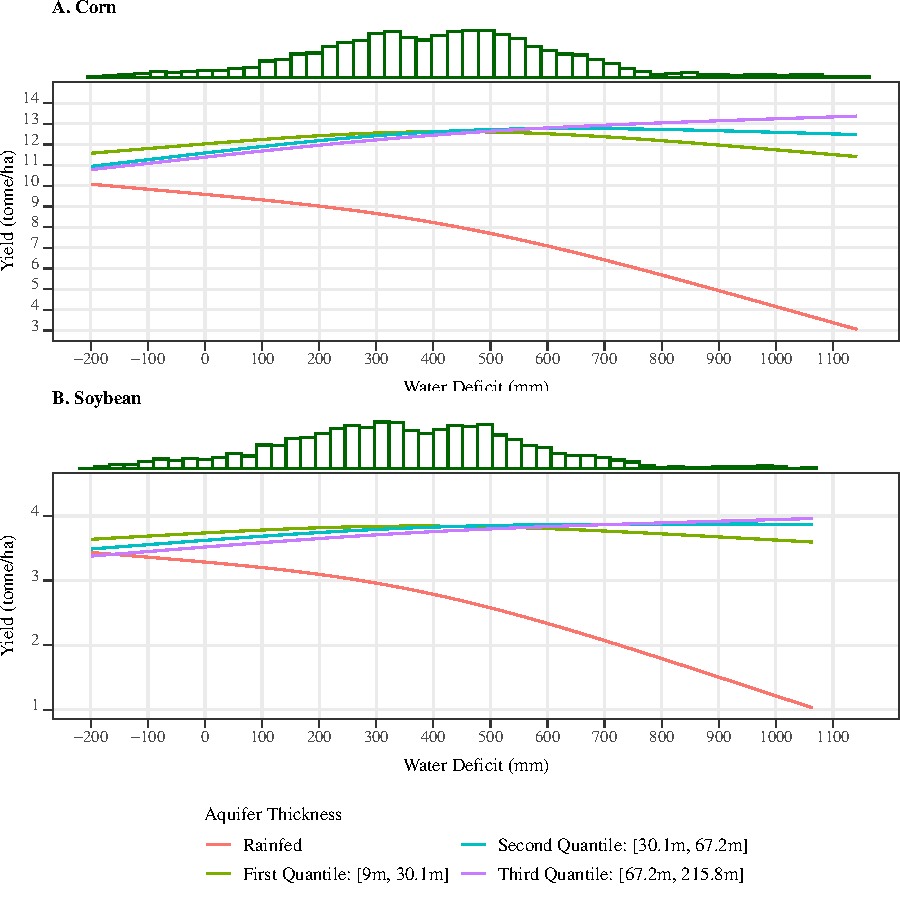
\includegraphics[width=6.5in,height=500px,]{../../Figures/g_yield_intensive} 

}

\caption{The impact of water deficit and aquifer thickness on rainfed and irrigated per-area yields of corn and soybean in US High Plains. Irrigated yield responses to water deficits are dissagregated by aquifer thickness level, considering three quantile groups that capture the range of aquifer thickness values in our sample: (i) 9 m to 30.1 m; (ii) 30.1 m to 67.2 m; and (iii) 67.2 m to 215.8 m. The histograms on the top of each panel show the distribution of county-level annual water deficit values included in regressions for each crop. Total number of observations are $8,773$ and $5,977$ for corn and soybean regressions, respectively.}\label{fig:yield-response}
\end{figure}

\begin{figure}[H]

{\centering 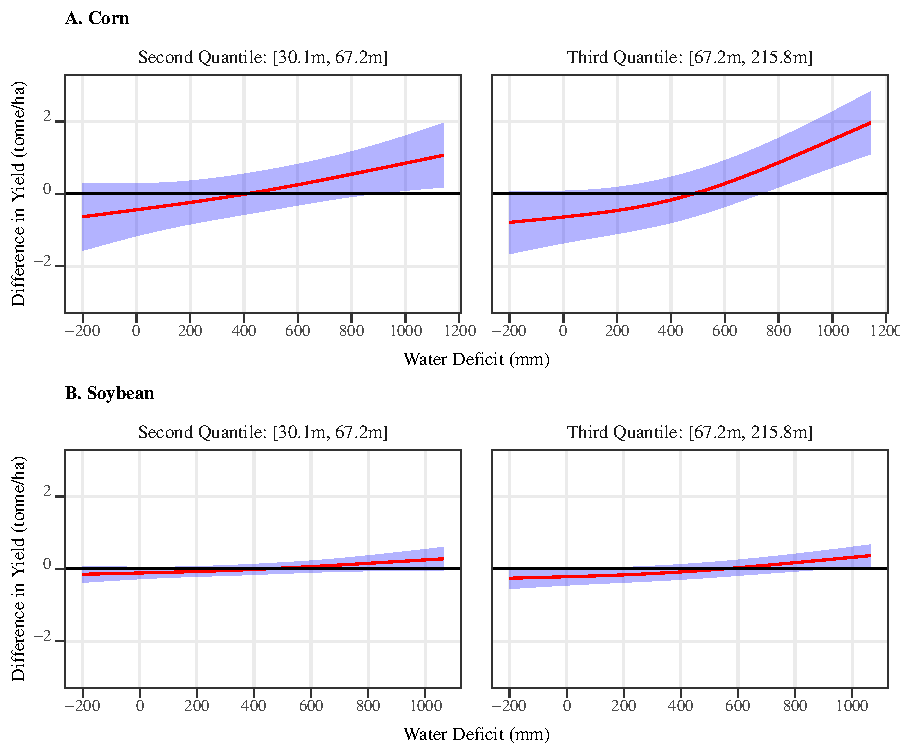
\includegraphics[width=6in,height=500px,]{../../Figures/g_ir_yield_dif} 

}

\caption{The difference in estimated county-level irrigated corn (top panels) and soybean (bottom panels) yields for counties in the second and third (largest) aquifer thickness quantiles relative to the first (smallest) aquifer thickness quantile.}\label{fig:yield-dif}
\end{figure}

\hypertarget{impact-share}{%
\subsection{Aquifer depletion substantially reduces the share of agricultural land under irrigation}\label{impact-share}}

While aquifer thickness has a statistically significant impact on per-area irrigated crop yields in drought conditions (water deficit greater than 700 mm), the magnitude of the yield impact is small when compared to differences between irrigated and rainfed production for the same weather conditions. One explanation for this result is that farmers may choose to retain a smaller proportion of land in irrigated production, so that limited groundwater pumping capacity can be used to adequately buffer crops against drought on land that remains under irrigation. Reductions in irrigated areas as an aquifer is depleted have been demonstrated theoretically \citep{rad2020effects, foster2014modeling, hrozencik2017heterogeneous, deines2020transitions}, but there has been little empirical research on farmers' irrigated area choices or how these are affected by combinations and magnitudes of weather risks and groundwater scarcity.

Figure \ref{fig:ir-share} shows the estimated relationship between aquifer thickness and the share of production area that is irrigated for corn and soybean after accounting for spatio-temporal variations in weather conditions and drought risk exposure across the aquifer. Figure \ref{fig:ir-share} demonstrates that aquifer thickness has meaningfully large impacts on the share of irrigated production for both corn and soybean. As aquifer thickness declines, the share of irrigated acres for corn decreases from around 0.90 (90\%) for an average county-level aquifer thickness of 100 m to 0.72 (72\%) for an average county-level aquifer thickness of 10 m (See Appendix \ref{test-dif-share} for formal statistical testings). Reductions in the share of production area under irrigation is also evident for soybean.

\begin{figure}[H]

{\centering 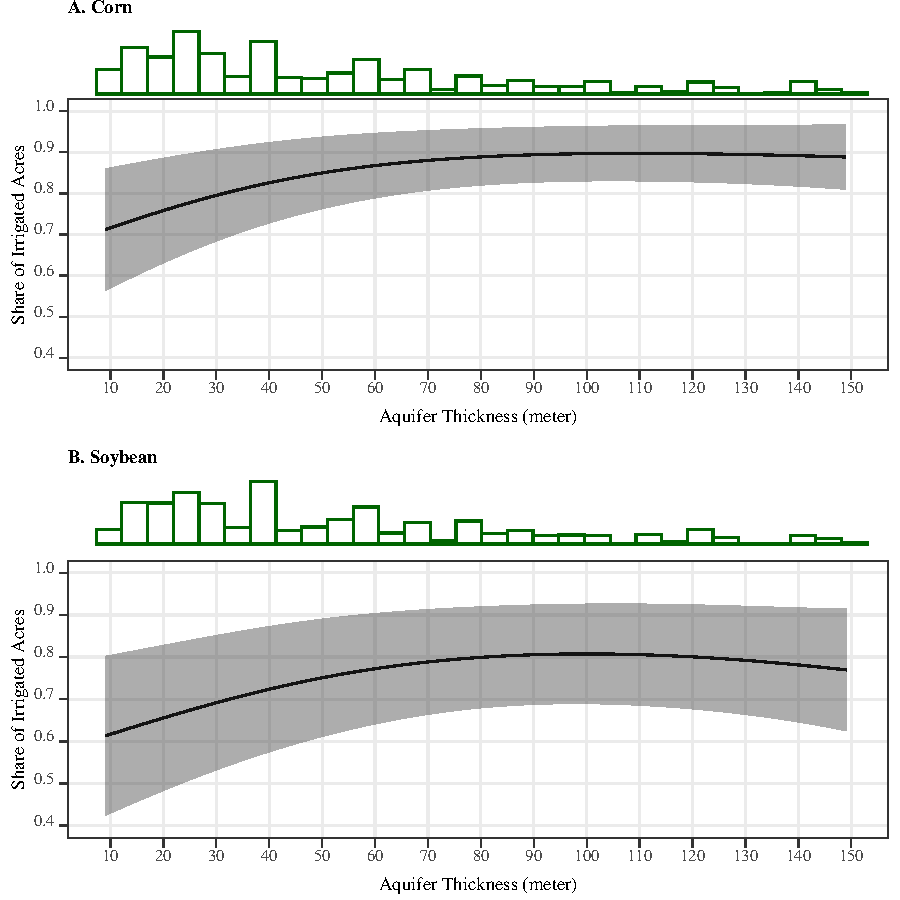
\includegraphics[width=6in,height=500px,]{../../Figures/g_share} 

}

\caption{The estimated impact of aquifer thickness on the share of agricultural production under irrigation for corn and soybean producing counties in the US High Plains (Note: shaded area represents 95\% confidence interval). The histograms on the top of each panel show the distribution of county-level aquifer thickness values included for each crop. Total number of observations are $2,523$ and $1,558$ for corn and soybean regressions, respectively.}\label{fig:ir-share}
\end{figure}

\hypertarget{aquifer-depletion-increases-overall-drought-related-production-losses-by-up-to-25}{%
\subsection{\texorpdfstring{Aquifer depletion increases overall drought-related production losses by up to \(25\%\)}{Aquifer depletion increases overall drought-related production losses by up to 25\textbackslash\%}}\label{aquifer-depletion-increases-overall-drought-related-production-losses-by-up-to-25}}

The overall influence of aquifer depletion on drought-related production losses is a function of both per-area irrigated yield and irrigated area changes highlighted in Sections \ref{impact-intensive} and \ref{impact-share}. Combining both responses, Figure \ref{fig:tot-impact} shows the relationship between water deficit and average per-area production (weighted-average of irrigated and rainfed yields, where the weights are production area shares) for corn and soybean at four values of aquifer thickness: 10, 40, 70, and 100 meters. While similar trends are observed as in Figure \ref{fig:yield-response}, the difference in production loss caused by high water deficits among the aquifer thickness levels are much more pronounced due to lower estimated irrigated area share for smaller aquifer thickness values. For example, for an aquifer thickness of 10 m, reductions in average yields occur for smaller water deficits than are required to trigger reductions in per-area irrigated yields alone. Similarly, the overall magnitude of yield reduction is greater for average yields than for per-area irrigated yields. This is because low aquifer thickness values have a greater estimated share of crop area under rainfed production, which magnifies average yield declines with increasing water deficits. 

Figure \ref{fig:dif-tot-impact} shows the difference in average per-area productivity for 40 m, 70 m, and 100 m aquifer thickness levels relative to an aquifer thickness of 10 m for corn and soybean. For corn, aquifer thickness does not have a significant impact on productivity when water deficits are below about 400 mm. However, beyond this threshold, higher levels of water deficit result in noticeable and statistically significant reductions to average corn production. This reflects the combination of lower irrigated yields under drought conditions, and, more importantly, reduced overall productivity due to smaller share of land under irrigation in areas where aquifer thickness is lower. Similar effects are also observed for soybean, although reductions in average production only occur at a higher deficit threshold (greater than around 600 mm) and are smaller in overall magnitude. For example, for a seasonal water deficit of 950 mm (average water deficit in 2012, the most extreme drought in our historical record), average per-area corn and soybean productivity are about 25\% and 15\% lower, respectively, when differentiating between areas with the 100 m and 10 m aquifer thicknesses.

Figure \ref{fig:tot-impact} and Figure \ref{fig:dif-tot-impact} also demonstrate that impact of aquifer thickness on average per-area production is highly non-linear at high seasonal water deficits. At a water deficit of 950 mm, for example, reducing from 100 m aquifer thickness to 70 m (decline of 30 m) would result in only 0.09 tonne/ha of production loss for corn. This negligible difference in average yield from the decline is due to the insensitivity of the share of irrigated acres to a decline in aquifer thickness when the initial aquifer thickness level is high as can be seen in Figure \ref{fig:ir-share}. Reducing from 70 m aquifer thickness to 40 m (decline of 30 m) would result in 0.95 tonne/ha of production loss for corn, with a further drop from 40 m aquifer thickness to 10 m (decline of 30 m) leading to 1.57 tonne/ha of production loss for corn. Similar but less pronounced effects are also observed for soybean. This non-linear impact of aquifer thickness is due to the influence of aquifer thickness on the share of irrigated corn acres (Figure \ref{fig:ir-share}), which implicitly reflects how aquifer thickness alters well yields and, in turn, farmers' ability to effectively and reliably buffer crops against water deficits during the growing season.  

\begin{figure}[H]

{\centering 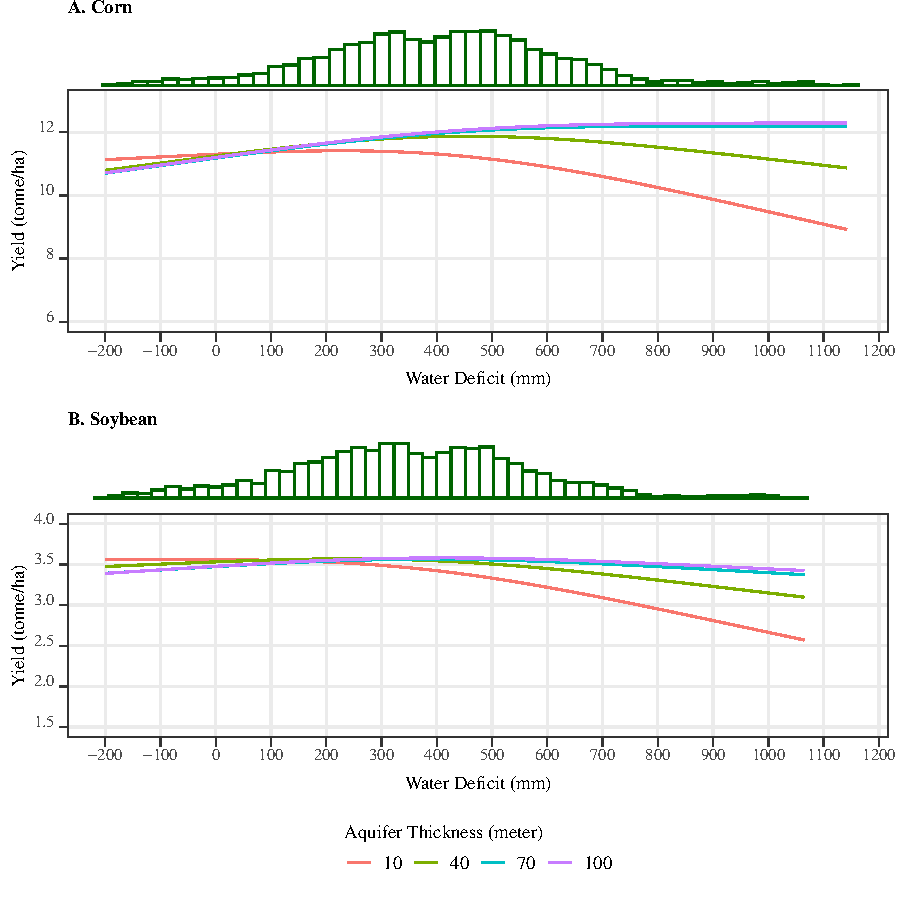
\includegraphics[width=6in,height=500px,]{../../Figures/g_total_impact} 

}

\caption{Average productivity of corn and soybean in the US High Plains for different levels of water deficit and aquifer thickness, considering both per-area yield responses and farmers' choices about irrigated area shares in response to different water deficit and aquifer conditions. See Appendix \ref{reg-conf} for estimated average yield response curves with 95\% confidence intervals displayed, which are omitted here for visual clarity.}\label{fig:tot-impact}
\end{figure}

\begin{figure}[H]

{\centering 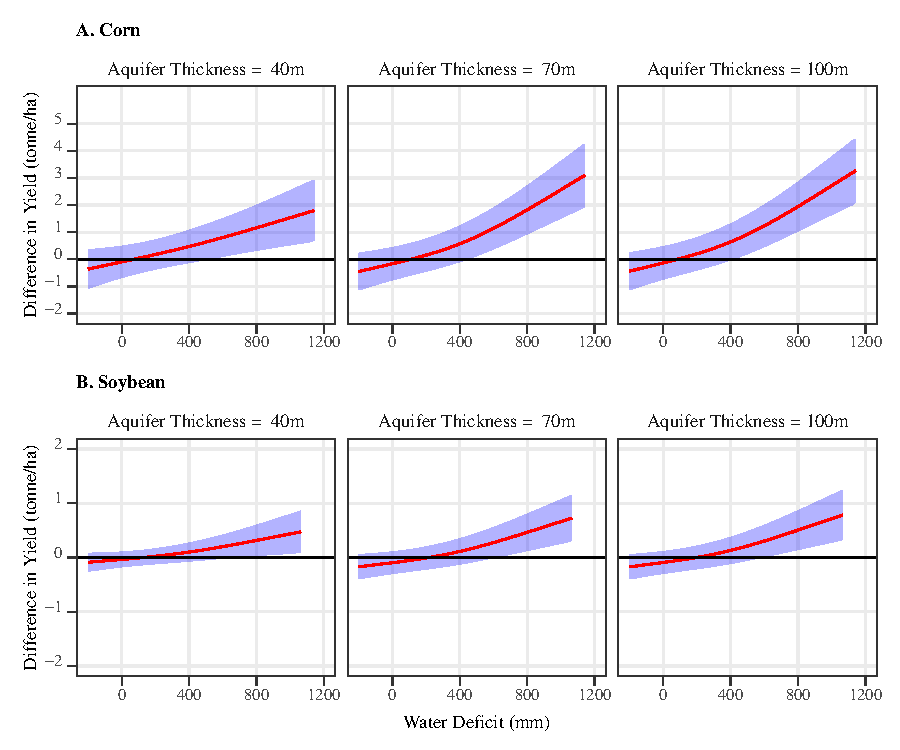
\includegraphics[width=6in,height=500px,]{../../Figures/g_avg_yield_dif} 

}

\caption{Difference in average yield of corn and soybean for aquifer thickness levels of 40 m, 70 m, and 100 m, relative to a baseline aquifer thickness of 10 m. Shaded areas denote 95\% confidence interval, which when greater than zero indicate average yields for the given aquifer thickness level are statistically significantly greater than for an aquifer thickness of 10 m at the 5\% level of significance.}\label{fig:dif-tot-impact}
\end{figure}

\clearpage

\hypertarget{discussion}{%
\section{Discussion}\label{discussion}}

We demonstrate the important role of aquifer thickness in determining farmers' ability to successfully buffer crops against drought risks in groundwater irrigated agricultural systems such as the High Plains of the United States. Previous research focused on impacts of drought on agricultural systems has largely focused either on risks for rainfed production \citep{schlenker2009nonlinear, lobell2014greater, schlenker2010robust, zhou2020connections, borgomeo2020impact} or for irrigated lands where water supply constraints are assumed to be minimal \citep{kuwayama2019estimating, zipper2016drought, zhu2022untangling, zhu2022warming, lu2020mapping, davis2019sensitivity, li2018changes, luan2021combined}. Our analysis adds new empirical insights to this literature by quantifying how reductions in aquifer thickness increase the vulnerability of irrigated agricultural production areas to drought events. Critically, our findings suggest that commonly adopted binary definitions of agricultural land areas into rainfed and irrigated categories are likely to underestimate exposure of crop production to drought risks, in particular in areas where water supplies for irrigation are insufficient to fully meet crop water needs in all years due to constraints imposed by hydrology, policies, and/or economics.

An important implication of our findings is that depletion of groundwater resources is likely to increase significantly the vulnerability of agricultural production to current and future drought risks. Climate change is projected to increase the frequency and severity of extreme drought events in many parts of the world \citep{ukkola2020robust, chiang2021evidence, cook2020twenty}, including in parts of Kansas and Texas \citep{bradford2020robust, cook2022projected, mullens2019quantitative} where the High Plains Aquifer continues to experience prolonged and significant declines in aquifer thickness \citep{scanlon2012groundwater, haacker2016water, cotterman2018groundwater}. Similar trends of increasing drought risks coupled with declining aquifer storage have been reported in other major groundwater irrigated farming systems worldwide \citep{wada2010global, doll2014global, famiglietti2014global, feng2018groundwater, bierkens2019non}. Our findings suggest that these simultaneous changes in aquifer conditions will amplify impacts of future climate change on crop production, with associated ramifications for resilience of supply chains, commodity markets, rural economies, and food security.

Our findings also provide useful guidance for water managers and policymakers seeking to address unsustainable groundwater use in the US High Plains and globally. Consistent with prior theoretical modeling, we demonstrate that the relationship between aquifer thickness and climatic water deficits during the growing season is highly non-linear when accounting for farmers' decisions about irrigated production areas. This indicates that sustainable groundwater conservation efforts \citep{macewan2017hydroecon, butler2020charting, elshall2020groundwater} should be targeted in space and time to avoid depletion exceeding critical thresholds which impair farmers' ability to effectively buffer production against drought. Analysis such as ours can provide valuable evidence about these critical thresholds and tipping points to guide proactive management of groundwater stocks, and, in doing so, limit economically damaging transitions from irrigated to rainfed production \citep{foster2017effects, deines2020transitions}. For example, several groundwater management agencies in the Texas portion of the HPA have in recent years set out targets to ensure 50\% of current aquifer storage and thickness remains in 50 years time (so called 50/50 rule) \citep{closas2018chronicle}. The effectiveness of such targets could likely be improved substantially by setting conservation targets based on empirical evidence about the level of aquifer thickness that is required to ensure adequate levels of drought protection, both now and with future climate change.

Several opportunities exist for future research to build upon the methods and analyses presented here. First, due to the limited resolution of our observational data, we were only able to estimate the impacts of different aquifer thickness categories on drought risk. Availability of sub-county crop yield data, for example from satellite remote sensing and/or in-situ monitoring \citep{edreira2020combining, deines2021million}, would allow models of the continuous effect of aquifer thickness on drought risk to be developed. Unobserved variations in aquifer properties will also introduce noise into the relationships between aquifer thickness, well yields, and drought risk. For example, a thinner aquifer interval composed of coarse sands and gravels may be able to supply comparable or higher well yields than a thicker aquifer dominated by fine sands and silt deposits, and hence offer greater resilience to water deficits despite similar or larger aquifer thickness \citep{butler2013interpretation, korus2020depletion}. These measurement errors in the relationship between aquifer thickness and well yield will lead to attenuation bias \citep{bound1991extent, hyslop2001bias}, suggesting that our analysis is likely to be an underestimate of the true impacts of groundwater depletion on drought risk. Nonetheless, our analysis shows that - even in the presence of these measurement uncertainties - we are still able to identify statistically significant increases in drought risk exposure for irrigated agriculture as a function of declining aquifer thickness. Improved data on spatial variations in aquifer properties and greater monitoring of real-world changes in well capacities alongside traditional water level measurements would help to further refine understanding of patterns of drought vulnerability across the HPA. This would enable more precise estimates to be made of critical tipping points in the resilience of irrigated agriculture to drought, which are needed to effectively design and target groundwater conservation policies.

Second, our analysis considered the effects of aquifer thickness on farmers' decisions to switch from irrigated to rainfed production, but did not assess other potential responses to aquifer depletion such as changing crop types or irrigation management practices. Switching to more drought resistant crops or varieties may enable farmers to maintain irrigated production at lower levels of aquifer thickness, and has been shown to be an important response to increasing agricultural water scarcity and abstraction policies in other studies \citep{bhattarai2021impact, deines2019quantifying, manning2017producer}. Improvements to irrigation scheduling practices and technologies, such as have been implemented as part of the SD6-LEMA (Local Enhanced Management Area) in Kansas \citep{deines2019quantifying, glose2022quantifying} and in parts of Texas \citep{mrad2020peak} and which are proposed as part of California's Sustainable Groundwater Management Act (SGMA) \citep{berbel2019droughts, lubell2020sustainable}, could also help to improve the efficiency of irrigation and, hence, the ability to more effectively meet crop water demands with lower well capacities. Such interventions may reduce - but not eliminate - increases in drought risk caused by lower or declining aquifer thickness, and could also help to mitigate against potential yield losses caused by over-use of water in wetter years via raising awareness of efficiency saving potentials \citep{foster2019assessing} and the importance of conservation \citep{marston2022}. However, risks also exist that irrigation efficiency improvements will increase net extraction, ultimately causing a rebound effect that exacerbates future aquifer depletion and drought risks \citep{grafton2018paradox,perez2021agricultural}. Future research should explore potential strategies that farmers could adopt to lessen the combined impacts of drought and aquifer depletion, alongside efforts to curb unsustainable groundwater extraction and climate change.

Finally, we focus on the impacts of aquifer thickness on agricultural resilience to seasonal water deficits. However, where water deficits are distributed unevenly during the season, negative impacts of aquifer depletion may be even larger. This is because reductions in well yields caused by aquifer depletion will constrain farmers' ability to meet peak crop water demands, increasing yield losses compared with if water deficits had been distributed evenly throughout the season \citep{ortiz2019unpacking}. Furthermore, irrigation also has broader benefits for crops such as reducing heat-related stress through cooling of land surface temperatures \citep{adegoke2003impact, bonfils2007empirical, lobell2008effect, zhu2022untangling}. Reductions in aquifer thickness therefore may have other negative impacts on irrigated crop productivity, if constraints to water supply due to aquifer depletion are significant enough to limit cooling benefits of irrigation during the growing season.

\hypertarget{methods}{%
\section{Methods}\label{methods}}

\hypertarget{data-sets}{%
\subsection{Data-sets}\label{data-sets}}

Our study focuses on the High Plains Aquifer (HPA) in the Central United States. Irrigated agriculture is integral to the landscape and economy of the HPA, with the region accounting for the majority of grain production in the United States valued in the billions of dollars annually \citep{smidt2016complex,fenichel2016measuring}. To evaluate the impacts of aquifer depletion on agricultural production overlying the HPA, we rely on data from several sources, which are described below.

County-level annual irrigated and rainfed yield data for corn and soybean for 1985 through 2016 were obtained from the U.S. Department of Agriculture's National Agricultural Statistics Service (USDA-NASS). USDA-NASS does not report irrigated yields disaggregated by the source of water used for irrigation. However, it is known that groundwater is the main source of water for irrigation for counties that overlie the HPA due to the limited availability of surface water resources in this area. Therefore, we retain both rainfed and irrigated yield observations for counties where greater than 75\% of the county area overlies the boundary of the HPA. For counties that do not meet this condition, only rainfed yield observations are obtained to avoid the possibility that irrigated production may be only partly dependent on use of groundwater from the HPA. We also include additional rainfed yield observations for counties that are outside the HPA, but within the main states covering the aquifer (i.e., South Dakota, Wyoming, Colorado, New Mexico, Nebraska, Kansas, and Texas), to enable more accurate estimation of the impact of drought for rainfed production as a point of comparison to our main irrigated crop yield analyses.

Meteorological data needed to estimate spatial and temporal variations in drought conditions across the HPA were obtained from the gridMET dataset \citep{Abatzoglou2013}. gridMET is a gridded daily weather dataset with a spatial resolution of \textasciitilde4km, and has been used in a range of climate impacts studies for agriculture and other sectors in the United States \citep{abatzoglou2016impact, pereira2015crop, crane2018machine, venkatappa2021impacts, zhu2019dissecting}. Daily precipitation values were extracted for each gridMET cell overlapping counties in our sample. Daily values of maximum and minimum temperature, surface radiation, wind speed, and humidity were also obtained from gridMET in order to calculate daily reference crop evapotranspiration for each grid cell. From these data, we computed the seasonal water deficit (\(D_{i,t}\)) for each grid cell by subtracting total precipitation from total reference evapotranspiration for the period May through September, which represents the typical growing season for corn and soybean in the HPA region. Seasonal water balance estimates were subsequently aggregated to the county-level to match our agricultural production data using an area-weighted average based on the proportion of the county covered by each overlapping gridMET cell. Figure \ref{fig:deficit-yield-hist} presents annual water deficit by year for the corn and soybean data, illustrating major drought events in the region in years such as 2000, 2002, and 2012. The importance of irrigation is clearly evident in years with large water deficits, with rainfed yields dipping substantially whereas irrigated yields are, on average, largely unaffected (Figure \ref{fig:deficit-yield-hist}).

Soil characteristics data (sand percentage, silt percentage, and water holding capacity) were obtained from the Soil Survey Geographic
Dataset (SSURGO). Observation units of the SSURGO data are polygons. For each county, the SSURGO polygons were overlaid with the county boundary, and the area-weighted average of the soil variables were calculated.

\begin{figure}[H]

{\centering 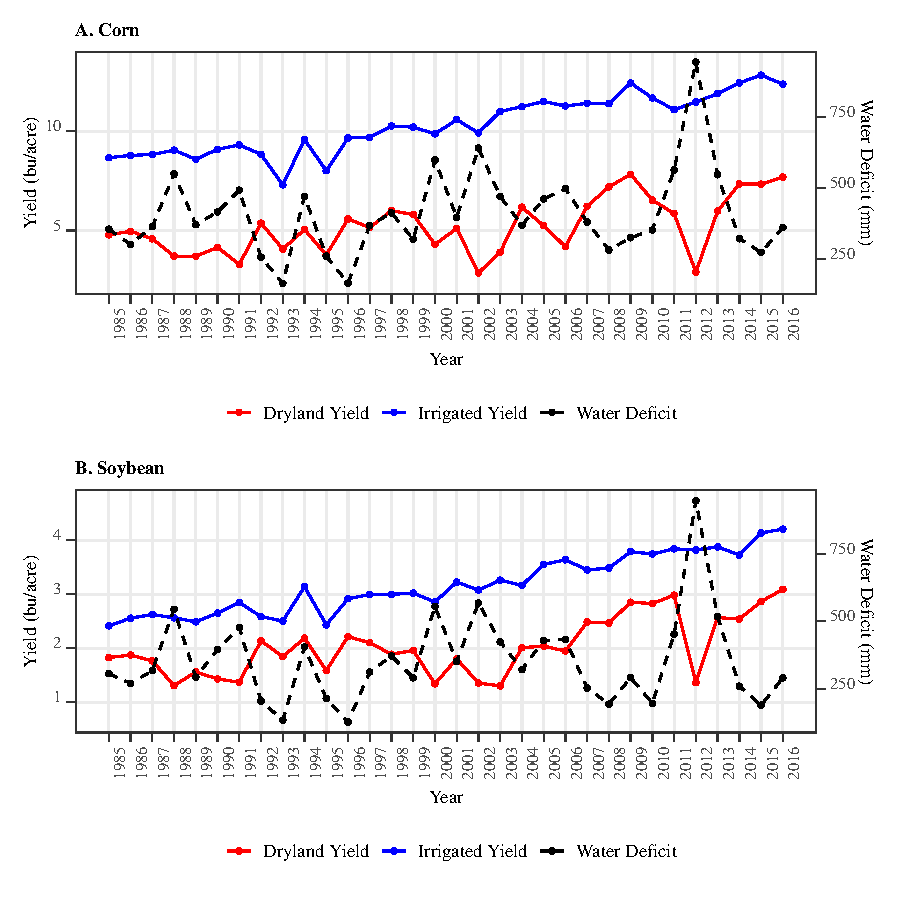
\includegraphics[width=750px,height=6in,]{../../Figures/g_y_wd_all} 

}

\caption{Historical rainfed yield, irrigated yield, and water deficit}\label{fig:deficit-yield-hist}
\end{figure}

As a proxy for the extent of aquifer depletion we use annual estimates of aquifer thickness generated by existing research \citep{haacker2016water,haacker2023}. These data provide annual estimates of the aquifer thickness at 250m resolution since 1935. Annual aquifer thickness maps were derived based on interpolation of 14,000 to 20,000 individual observations of water levels per year, along with detailed maps of both the land surface elevation and bedrock elevation of the HPA. Aquifer thickness estimates for each year were aggregated to the county level using an area-weighted average to match the resolution of agricultural production data. Aquifer thickness values were only estimated for counties with irrigated yield observations. Furthermore, during the aggregation process, any aquifer cells within a county that had a aquifer thickness value lower than 9 m were removed before aggregation to reflect the fact that aquifer thicknesses lower than this threshold are not considered to be viable for extraction and therefore it is unlikely these areas contribute groundwater for irrigation production \citep{fenichel2016measuring, haacker2016water, deines2020transitions}. Figure \ref{fig:sat-map} presents the distribution of aquifer thickness across our study area for counties included in corn and soybean analyses. Aquifer thickness levels vary substantially over space and time, which we will exploit in our analysis to quantify how aquifer thickness influences farmers' exposure and responses to drought.

These data were combined to form four sets of data for regression analysis: (1) per-acre corn yield ($8,773$ observations), (2) per-acre soybean yield ($5,977$ observations), (3) share of irrigated corn ($2,523$ observations), and (4) share of irrigated soybean ($1,558$ observations).

\begin{figure}[H]

{\centering 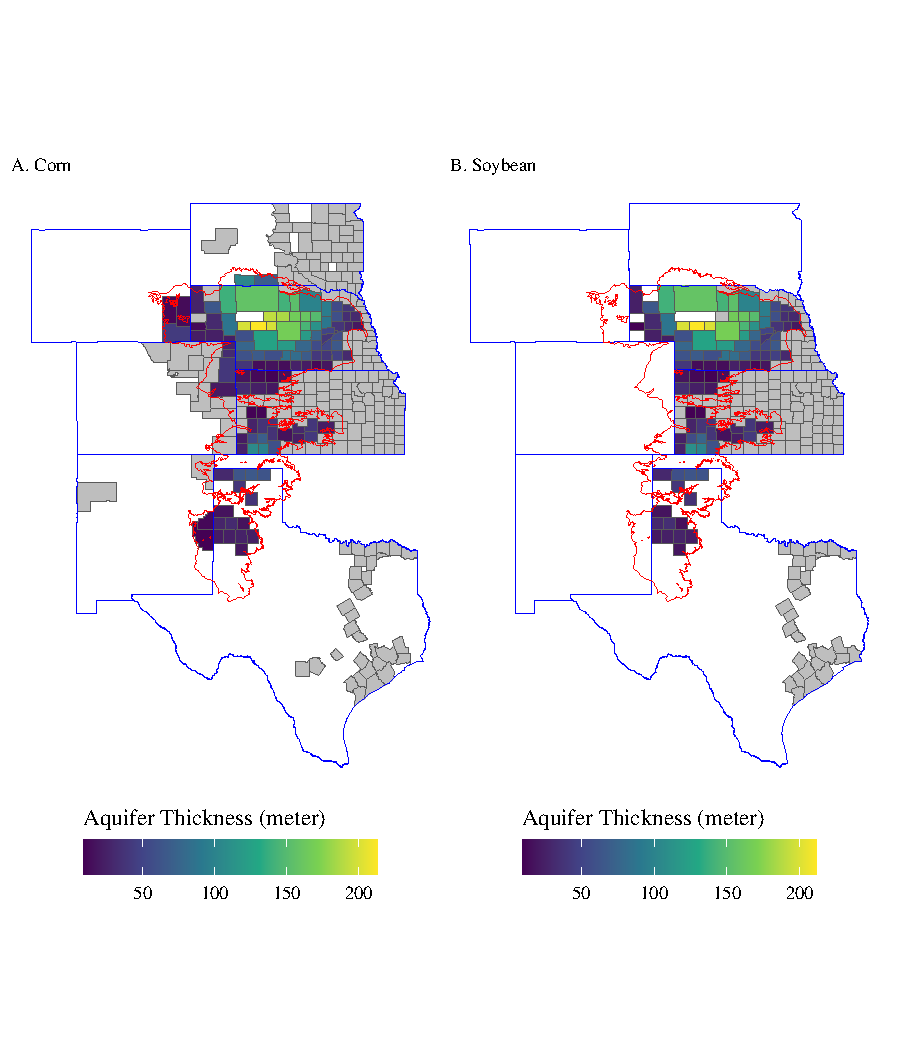
\includegraphics[width=6in,height=500px,]{../../Figures/g_map} 

}

\caption{Map showing county-average aquifer thickness in 2016 for each county included in our corn and soybean regression analyses. Counties highlighted in grey are rainfed only, and the red polygon denotes the boundary of the High Plains Aquifer system}\label{fig:sat-map}
\end{figure}

\hypertarget{regression-models}{%
\subsection{Regression Models}\label{regression-models}}

Aquifer depletion may impact resilience of irrigated crop production to drought through two main channels: (1) a reduction in per-area irrigated yields due to the economic or physical inability to meet crop water requirements; and (2) a reduction in the area of land irrigated, resulting in reduced production due to lower yields obtained through rainfed agriculture.

To assess the first of these impacts, we quantify the impact of seasonal water deficits (\(D\)) during the growing season (May through September) on county-level rainfed and irrigated yields (\(Y\)) using a hierarchical generalized additive model, where irrigated yield response to seasonal water deficits is conditioned on the level of aquifer thickness (\(A\)) in the county in a given year. Our regression model is given in Equation \eqref{eq:eqn1}, with the same model formulation used for corn and soybean:

\begin{equation}
Y_{i,t} = \sum_{j=1}^4 \sigma_j C_j + \sum_{j=1}^4 \sum_{k=1}^K \beta_{j,k}\phi_{j,k}(D_{i,t})\cdot C_j  + \alpha_i + \lambda_t + v_{i,t} \label{eq:eqn1}
\end{equation}

where county and year are indicated by subscripts \(i\) and \(t\), respectively, \(Y\) is crop yield, and \(D\) is seasonal water deficit. \(C_j\) is a dummy variable that takes 1 if observation \(i\) is under category \(C_j\), 0 otherwise. The observations are grouped into four categories: rainfed production, and county-years with aquifer thickness falling in the \([0\%-33.3\%)\), \([33.3\%-66.7\%)\), and \([66.7\% - 100\%]\) quantile ranges of aquifer thickness. The three irrigated production groups have about the same number of observations, which ensures statistical stability in estimating yield response to drought by category. Spline functions are used to capture the potential non-linearity of the impact of water deficit on yield in a flexible manner, with \(\sigma_j\) representing the category-specific intercept, \(\phi_{j,k}\) \(k\)th spline basis function, and \(\beta_k\) is its coefficient (see Appendix \ref{spline-basis} for further explanations on how spline-based regression works). $K$ is the total number of spline basis functions. $K = 3$ was chosen for this regression as it minimizes Bayesian Information Criterion (BIC). To control for time-invariant heterogeneity across counties and yearly shocks, county fixed effects (\(\alpha_i\)) and year fixed effects (\(\lambda_t\)) are also included and standard error estimation is clustered by county.

To estimate the additional impact of aquifer thickness on the share of total acres that are irrigated in a county, a fractional logit model under the generalized additive model framework is used in which the impact of aquifer thickness, average water deficit, and their interactions are estimated without the prior requirement to assume any functional forms. This allows for flexible representation of the non-linear relationships between drought risks, aquifer conditions, and agricultural land use, including potential thresholds in farmers' irrigated area choices under water supply constraints that have been noted in prior work \citep{foster2015well, foster2015analysis, hrozencik2017heterogeneous}. The model is given in Equation \eqref{eq:eqn2} below:

\begin{equation}
    log(\frac{s_{i,t}}{1-s_{i,t}}) = \beta_0 + \sum_{k=1}^K \eta_{k}\phi_{k}(D_{i}) + \sum_{l=1}^L \beta_{l}\tau_{l}(A_{i,t}) + X_i + \theta_{s,t} + v_{i,t} \label{eq:eqn2}
\end{equation}

where \(s_{i,t}\) is the share of irrigated production. The impact of average water balance is captured by \(\sum_{k}^K \eta_{k}\phi_{k}(D_{i})\), where \(\phi_{k}(\cdot)\) is the \(k\)th spline basis function and \(\eta_{k}\) is its coefficient. The impact of aquifer thickness is captured in a similar way with \(\tau_{l}(\cdot)\) and \(\beta_{l}\) being the \(l\)th spline basis function and its coefficient, respectively. $K$ and $L$ are the numbers of basis functions for $D$ and $A$, respectively. $K = 4$ and $L = 4$ were chosen as they minimize BIC. County-level soil characteristics including sand percentage, silt percentage, and water holding capacity, are represented by \(X_i\). State-year fixed effects and error term are represented by \(\theta_{s,t}\) and \(v_{i,t}\), respectively. Unlike for our regression models of per-area yields, we do not include county fixed effects to avoid eliminating the majority of variation in the aquifer thickness variable. The vast majority of variation in aquifer thickness is cross-sectional (across counties), rather than over time. Including county fixed effects would effectively eliminate the cross-sectional variation in aquifer thickness. A formal discussion of the trade-offs associated with the choice of fixed effects is provided in Appendix \ref{county-fe}.

In the final step of our analysis, we then estimate the average crop yield as a function of aquifer thickness and seasonal water deficit. The average crop yield is estimated as the average of rainfed and irrigated yields estimated on the basis of Equation \eqref{eq:eqn1}, weighted by the estimated share of total acres that are irrigated in the county estimated using Equation \eqref{eq:eqn2}. In this combined model, aquifer thickness is a continuous variable for the irrigated area share regression component and a categorical variable for the irrigated yield regression following the format of Equations \eqref{eq:eqn2} and \eqref{eq:eqn1}, respectively. Comparing the estimated average crop yield across different levels of aquifer thickness for a given seasonal water deficit provides an indication of the effect of aquifer conditions on drought impacts, considering impacts of drought through changes in both per-area irrigated yields and the area of land irrigated. Standard errors of this analysis are estimated using bootstrap methods clustered by county. Note that irrigated area share and average crop yield estimates use data only from counties that have both irrigated and rainfed production observations because irrigated area share cannot be calculated when missing either one of the irrigated and rainfed observations. Counties with solely irrigated or rainfed production observation data (Section \ref{data-sets}) are used solely for estimating impacts of drought on per-area crop irrigated or rainfed yields respectively (Equation \ref{eq:eqn1}).

\hypertarget{data-and-code-availability}{%
\subsection{Data and Code Availability}\label{data-and-code-availability}}

All the codes used for this study are available at the following Github repository (\href{https://github.com/tmieno2/Drought-Production-Risk-Aquifer}{link}). All analyses were performed in R \citep{R} and all the raw data-sets used in this study are publicly accessible. The boundary shape file of the High Plains aquifer was obtained from the U.S. Geological Survey at \url{https://water.usgs.gov/GIS/metadata/usgswrd/XML/ds543.xml#stdorder}. This data is used for Figure \ref{fig:sat-map}. Corn and soybean yield data were obtained from the U.S. Department of Agriculture's National Agricultural Statistics Service (USDA-NASS), available at \url{https://www.nass.usda.gov/Quick_Stats/}. The R tidyUSDA package \citep{RtidyUSDA} was used to automatically download the relevant data. This data is used for Figure \ref{fig:deficit-yield-hist} and the regression analysis. Weather data (precipitation, temperature, and evapotranspiration) was obtained from the gridMET dataset \citep{Abatzoglou2013}, which is available at \url{https://www.climatologylab.org/gridmet.html}. This data is used for Figure \ref{fig:deficit-yield-hist} and the regression analysis. The aquifer thickness data were obtained from Hydroshare \citep{haacker2023} available at \url{https://www.hydroshare.org/resource/7d925c7944244032af98c9ed20c22db6/}. This data is used for Figure \ref{fig:sat-map} and the regression analysis. Soil characteristics data was obtained from the Soil Survey Geographic Dataset, which is used for regression analysis. The R soilDB package \citep{Rsoildb} was used to download the data. Regression analyses are implemented using the R fixest package \citep{Rfixest}. Other key R packages include ggplot2 \citep{Rggplot2} for creating plots, data.table \citep{Rdatatable} for data wrangling, and sf \citep{Rsf} for spatial data operations. The data used for the regression analysis can be generated using our codes by following the instructions available at the linked Github repository.

\clearpage

\hypertarget{appendix-appendix}{%
\appendix}

\hypertarget{pathway-reg}{%
\section{Groundwater management policies as a potential causal pathway}\label{pathway-reg}}

Our analysis evaluates the links between aquifer thickness and drought resilience, proposing a causal link between declining aquifer thickness and irrigated production during droughts. In the first section of our manuscript, we propose that this connection is driven by impacts of aquifer thickness on well yields and, hence, farmers ability to use groundwater to fully buffer crops against water deficits during drought. 

It is important to assess the extent to which this causal relationship may be affected or confounded by other factors. One key alternative hypothesis is that regulations limiting groundwater withdrawals could have been introduced as a response to declining aquifer thickness, with resulting reductions in irrigated areas and irrigated crop yields driven by regulatory rather than hydrologic (i.e. well yield) constraints. Below, we discuss the reasons that regulatory constraints are highly unlikely to be the cause of the relationships between aquifer thickness and drought impacts observed in our analysis for the HPA. 

First, it is important the majority of groundwater withdrawal regulations that do exist in the HPA limit pumping to a specified volume over a multiyear period. It is also common for farmers to have been allowed to bank and carryover significant volumes of water deficits from historic periods when allocation levels were higher \citep{rimvsaite2023groundwater}, further increasing their regulatory quotas above defined caps. Together, these factors mean that farmers in parts of the HPA where groundwater withdrawals are regulated or restricted are still able to increase water withdrawals substantially in drought years when demand is higher. Prior research has shown that as a result farmers water use decisions in HPA are not constrained by such regulations even in extreme drought years such as 2012 \citep{foster2019assessing}.

Where more restrictive groundwater withdrawal limits have been introduced, for example in some Groundwater Management Districts in Kansas \citep{marston2022, rimvsaite2023groundwater}, these have universally been implemented in the last 5-10 years and therefore have no or only minimal overlap with our study period which extends up to only 2016. The earliest of these groundwater managements in Kansas interventions was the Sheridan 6 Local Enhanced Management Area (LEMA) in Northwest Kansas, which introduced restrictions to farmer groundwater pumping of 11 inches per year on average per 5-year period starting in 2013. While this overlaps with the final 4 years of our study period, the Sheridan 6 LEMA area covers only parts of two counties in Kansas and hence represents a very small proportion of our overall study sample. Additionally, the years 2013-2016 were all characterized by average or above average growing season rainfall (i.e. not drought years). Furthermore, evidence shows that the effect of restrictions introduced by the LEMA has primarily been a reduction in per-area water use, with irrigated crop yields largely unaffected and only small reductions in irrigated areas compared to pre-policy conditions \citep{drysdale2018adaptation, deines2021combining, whittemore2023108408}. These policies therefore would not be expected to confound our results on the impacts of aquifer thickness. 

Finally, we also highlight that areas of the southern HPA, in particular in northern Texas, where the lowest aquifer thickness values are observed have few if any regulatory restrictions on groundwater extraction. This is due to laws that typically provide farmers with absolute rights to use groundwater under their land, coupled with low levels of metering. Research has shown that these conditions have historically limited or constrained potential for implementing extensive and binding pumping restrictions on irrigators in these areas \citep{wheeler2016lessons, closas2018chronicle}, again indicating that regulations are not the binding driver of water use constraints in these areas. As discussed in section \ref{main} of our manuscript, there is extensive evidence pointing to reduced well yields in these areas of the HPA. This evidence ranges from anecdotal and theoretical insights to simulation-based studies. Collectively, they suggest that these restrictions significantly constrain farmers' ability to meet crop water demands during droughts.

\hypertarget{reg-conf}{%
\section{Uncertainties in estimated impacts of water deficit on irrigated and average yield}\label{reg-conf}}

\setcounter{figure}{0}
\renewcommand{\thefigure}{A.\arabic{figure}}

In the main article, the confidence intervals of the estimated yield responses to water deficit were not presented to enable easier comparison between response curves. This section provides visualization of yield response with the 95 \(\%\) confidence interval to convey the degree of uncertainty in our estimation. Figures \ref{fig:irrigated-yield-ind-corn} and \ref{fig:irrigated-yield-ind-soy} present the impact of water deficit on crop yield by aquifer thickness category with the 95\(\%\) confidence interval for irrigated corn and soybean, respectively. Figure \ref{fig:avg-yield-ind} presents the impact of water deficit on average crop yield (irrigated and rainfed combined) by aquifer thickness category for corn and soybean with the 95\(\%\) confidence interval.

\begin{figure}[H]

{\centering 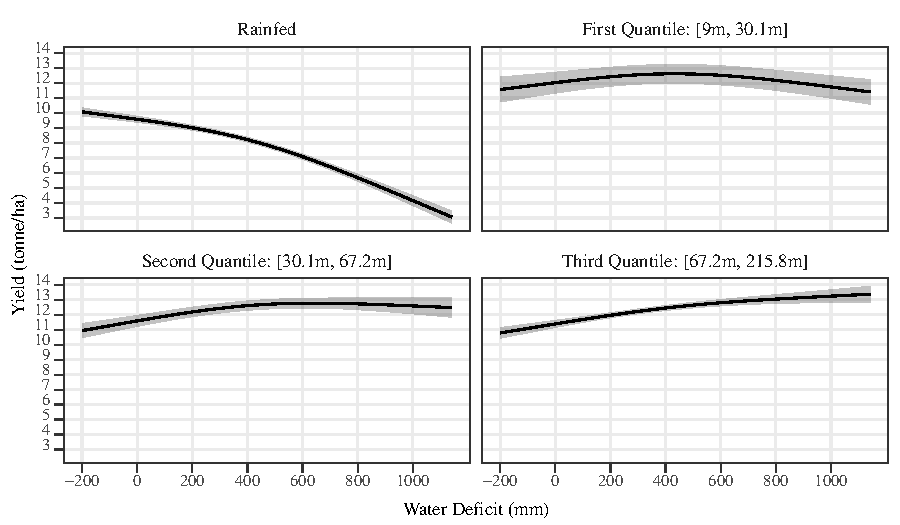
\includegraphics[width=6in,height=500px,]{../../Figures/g_yield_with_conf_corn} 

}

\caption{The impact of water deficit and aquifer thickness on rainfed and irrigated per-area irrigated yields of corn in US High Plains (solid black line) with 95\% confidence interval (grey shaded area)}\label{fig:irrigated-yield-ind-corn}
\end{figure}

\begin{figure}[H]

{\centering 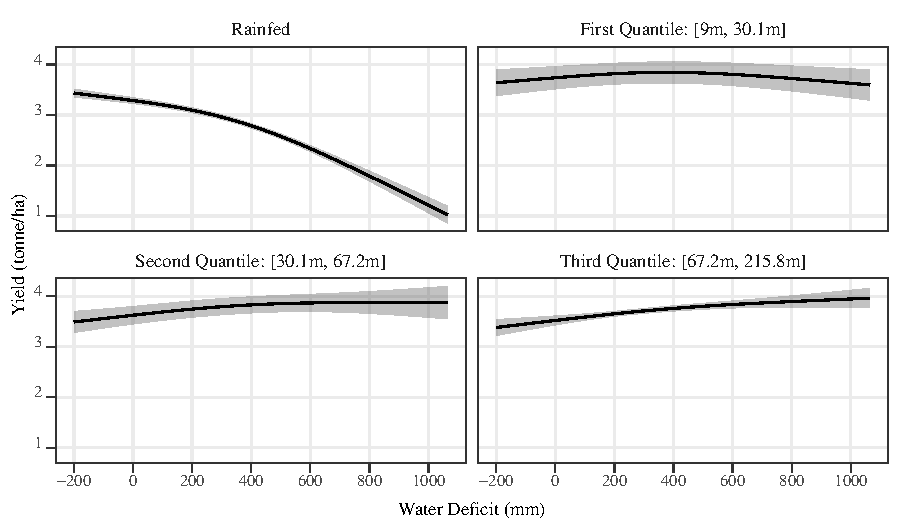
\includegraphics[width=6in,height=500px,]{../../Figures/g_yield_with_conf_soy} 

}

\caption{The impact of water deficit and aquifer thickness on rainfed and irrigated per-area irrigated yields of soybean in US High Plains (solid black line) with 95\% confidence interval (grey shaded area)}\label{fig:irrigated-yield-ind-soy}
\end{figure}

\begin{figure}[H]

{\centering 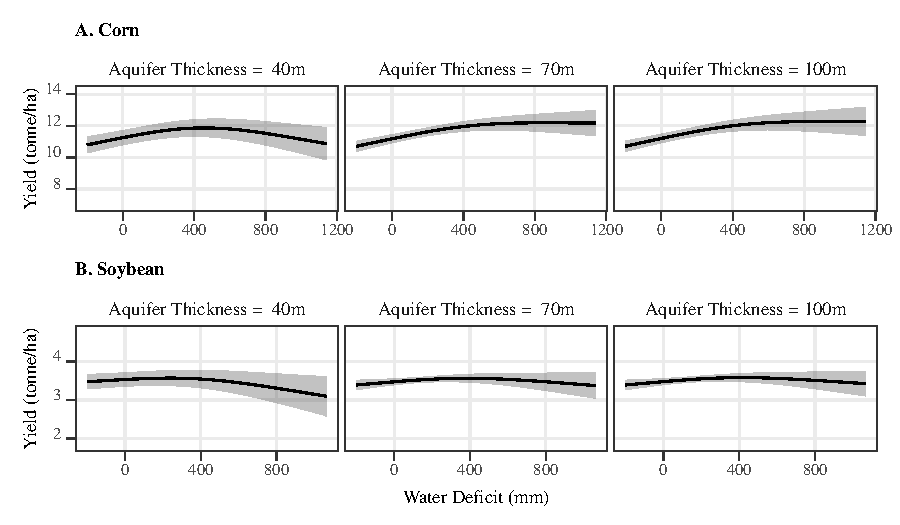
\includegraphics[width=6.5in,height=500px,]{../../Figures/g_avg_yield} 

}

\caption{Average productivity of corn and soybean in the US High Plains for different levels of water deficit and aquifer thickness (solid black line) with 95\% confidence interval (grey shaded area)}\label{fig:avg-yield-ind}
\end{figure}

\clearpage

\hypertarget{test-dif-share}{%
\section{Comparison of the impacts of different aquifer thickness levels on irrigated area share}\label{test-dif-share}}

\setcounter{figure}{0}
\renewcommand{\thefigure}{B.\arabic{figure}}

Figure \ref{fig:test-sat-share} presents the difference in the estimated share of irrigated acres at different levels of aquifer thickness relative to the aquifer thickness level of 100 m, which represents a high level of aquifer thickness for our study area that exerts no constraints on water supply for irrigation. Grey shaded areas represented the 95\% confidence intervals for the estimated relationships. Where this range exceeds the red zero line, this indicates that the difference in aquifer thickness (relative to 100 m baseline) leads to a statistically significant (at 5\% level) reduction in irrigated production area share. 

\begin{figure}[H]

{\centering 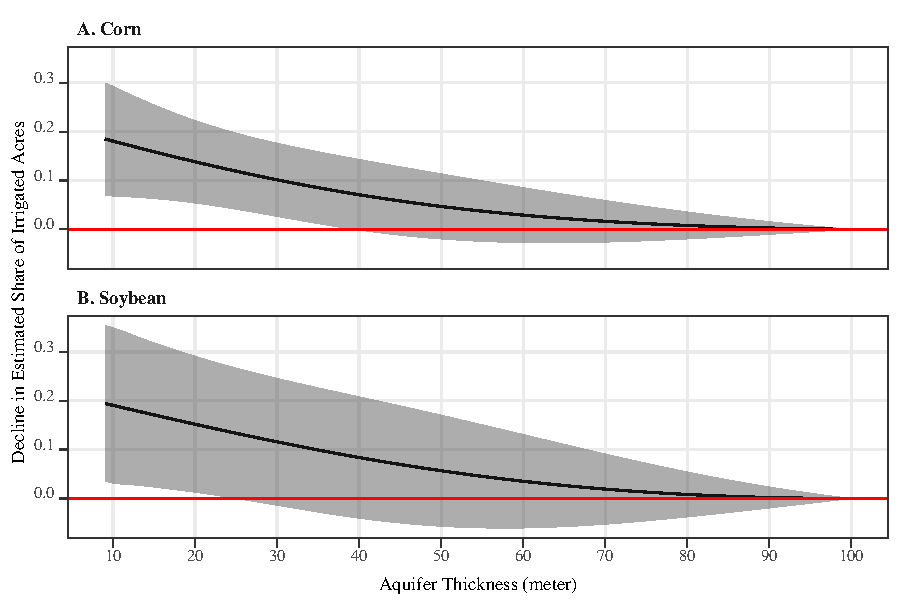
\includegraphics[width=6.5in,height=500px,]{../../Figures/g_share_dif} 

}

\caption{Decline in the share of acres that are irrigated as a function of different levels of aquifer thickness relative to a baseline aquifer thickness level of 100 m (black line). The grey shaded areas represent the 95\% confidence interval for this estimated relationship.}\label{fig:test-sat-share}
\end{figure}

\clearpage

\hypertarget{county-fe}{%
\section{Comparison of the choice of spatial fixed effects in irrigation area share regressions}\label{county-fe}}

\setcounter{figure}{0}
\renewcommand{\thefigure}{C.\arabic{figure}}

Figure \ref{fig:variation-left} presents the histogram of aquifer thickness after demeaning these values by removing either their: (A) yearly average, (B) state-year average, or (C) county average values. This analysis is used to gain insights into how much variation in aquifer thickness for identification is left when implementing either: (A) only year fixed effects, (B) state-year fixed effects, or (C) county and year fixed effects. As shown in Figure \ref{fig:variation-left}, including state-year fixed effects does not substantially reduce the total variation in aquifer thickness compared to including only year fixed effects. However, including county fixed effects dramatically reduces the total variation in aquifer thickness, resulting in extremely inaccurate estimates of impacts of aquifer conditions on drought risk (high standard error). For this reason, we included state-year fixed effects in our irrigated production share regression analysis to strike a balance between preserving variability in aquifer thickness data and ensuring controls for other unobserved spatial factors that may influence estimates of the impacts of aquifer conditions on production shares. 

\begin{figure}[H]

{\centering 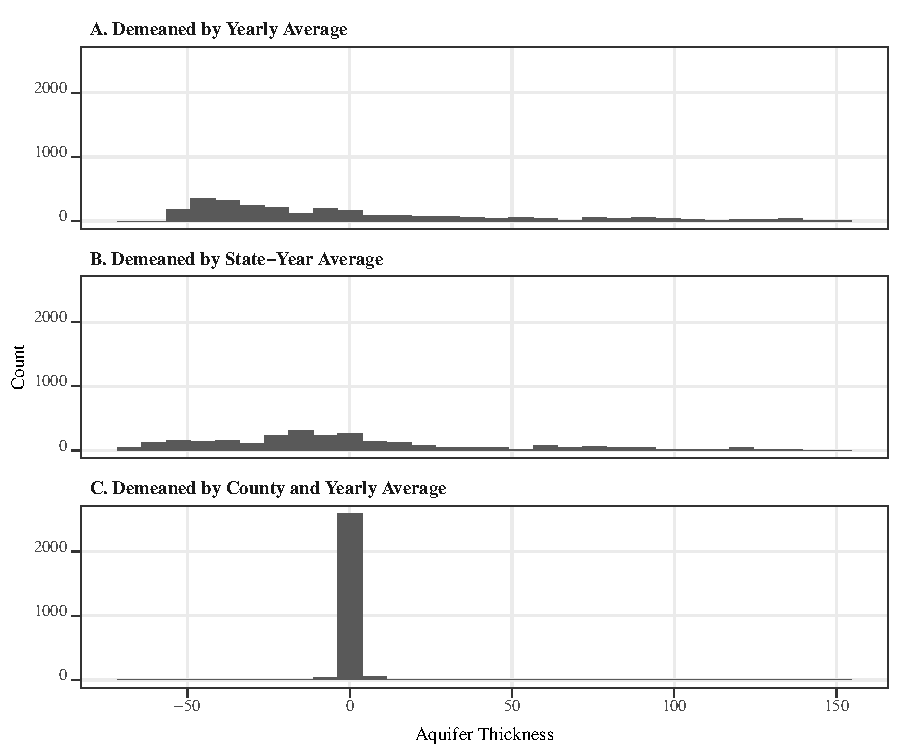
\includegraphics[width=6in,height=500px,]{../../Figures/g_variation} 

}

\caption{Comparison of variations in aquifer thickness after demeaning by yearly average, state-year average, and county average.}\label{fig:variation-left}
\end{figure}

Figure \ref{fig:state-fe-with-without} compares the impact of aquifer thickness on the share of irrigated acres for corn and soybean with different sets of fixed effects. For both corn and soybean, the negative impact of a reduction in aquifer thickness on the share of irrigated acres is virtually the same when using different possible sets of fixed effects. Importantly, adding state-year fixed effects, which control for unobservables at the state-year level, does not alter the estimated impacts of aquifer thickness on share of acres irrigated. This indicates that, even though there may be unobservables that are spatially correlated with aquifer thickness beyond soil characteristics, their correlation may not cause significant bias to our estimation and findings. We note that more detailed assessment of the impacts of including county-fixed effects is beyond the scope of our available datasets, and we defer this matter to future studies where greater temporal variations in aquifer thickness levels may be available to allow incorporation of county-level fixed effects.

\begin{figure}[H]

{\centering 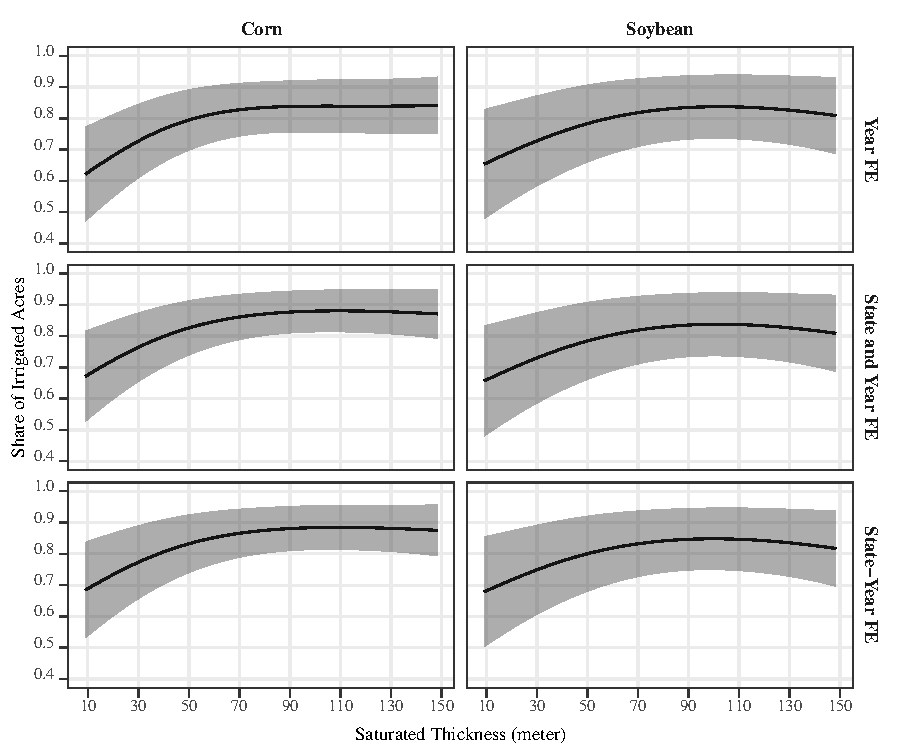
\includegraphics[width=6in,height=500px,]{../../Figures/g_share_comp} 

}

\caption{Comparison of estimated impact of aquifer thickness on the share of irrigated acres with and without state fixed effects}\label{fig:state-fe-with-without}
\end{figure}

\clearpage

\hypertarget{spline-basis}{%
\section{Spline basis functions and GAM estimation}\label{spline-basis}}

\setcounter{figure}{0}
\renewcommand{\thefigure}{D.\arabic{figure}}

We used generalized additive models (GAM) for our regression analysis. In GAM, the impact of a variable on the dependent variable can be expressed as a series of spline basis functions and their coefficients. Suppose you are interested in modeling the following model.

\begin{equation}
y = f(x) + \mu
\end{equation}

Where \(f(x)\) represents the impact of variable \(x\) on \(y\). The shape of \(f(x)\) is not known to the researcher. GAM attempts to represent \(f(x)\) with a series of spline basis functions and their coefficients like below.

\begin{equation}
y = \sum_{k=1}^K \beta_k \phi_k(x) + \mu
\end{equation}

Where \(\phi_k(\cdot)\) is the \(k\)th spline basis function and \(\beta_k\) is its coefficient. Figure \ref{fig:sp-basis} provides a visual illustration of a series of thin-plate spline basis functions.

\begin{figure}[H]

{\centering 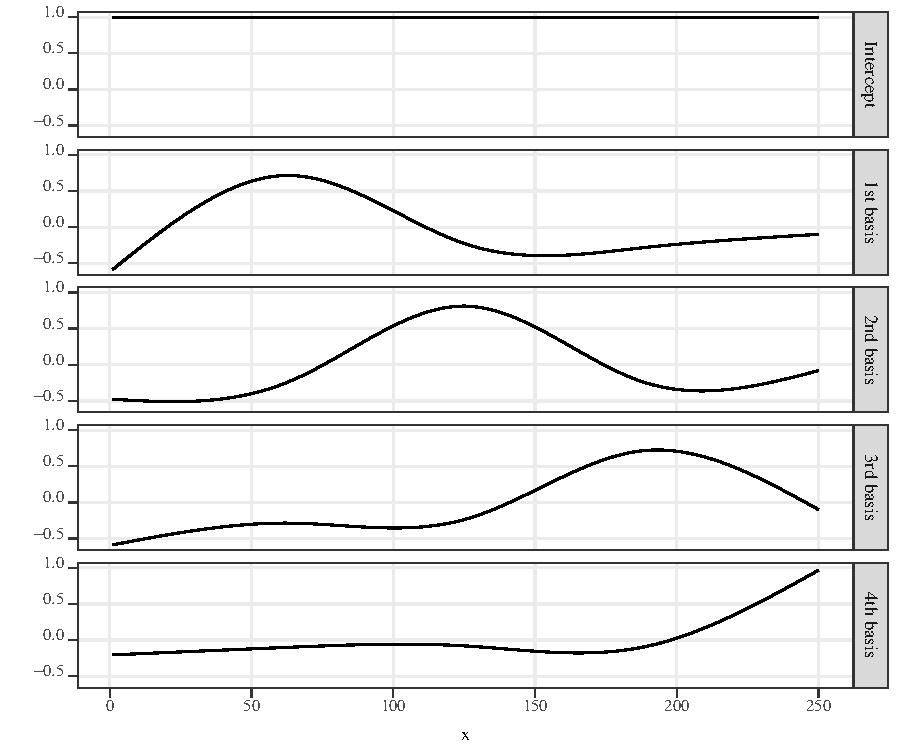
\includegraphics[width=6in,height=500px,]{../../Figures/g_basis} 

}

\caption{Example of a series of thin-plate spline basis functions}\label{fig:sp-basis}
\end{figure}

Different coefficients (or namely weights) given to the spline basis functions result in different shapes of the impact of \(x\) on \(y\). Figure \ref{fig:ex-fx} presents two examples of two different sets of coefficients and their resulting representation of \(f(x)\). In the first case, \(\{\beta_1, \dots, \beta_5\} = \{60, 60, 60, 60, 60\}\). In the second case, \(\{\beta_1, \dots, \beta_5\} = \{20, -20, -40, 40, 60\}\). Among all the possibilities of the combinations of the coefficients, GAM finds the set of coefficient values that fits the data best. Unlike non-parametric regression, a GAM is a linear (in-parameter) model and estimates $\beta_k$ to best fit the observation data.

\begin{figure}[H]

{\centering 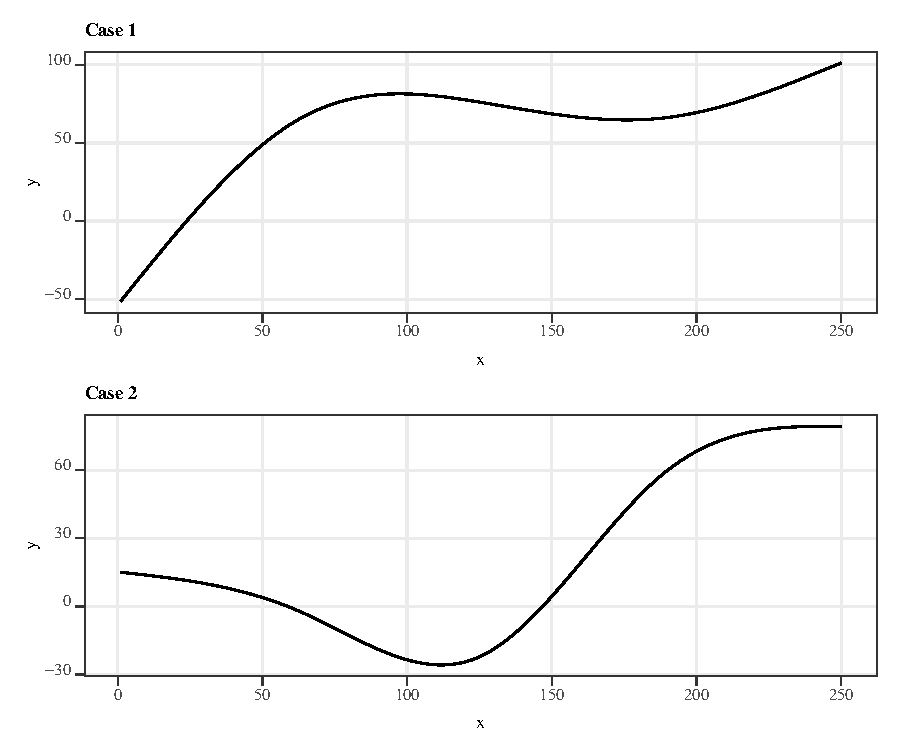
\includegraphics[width=6in,height=500px,]{../../Figures/g_il_y} 

}

\caption{Example of a function represented by different coefficient values}\label{fig:ex-fx}
\end{figure}

\clearpage

  \bibliography{DRA.bib}

\end{document}
